% ..............................................................................
% FAU Beamer Presentation: 6G Tower Placement Optimization
% Meeting 2: System Architect Presentation
%
% Based on the fau-beamer template by Tim Roith <tim.roith@fau.de>
% ..............................................................................

\documentclass[final]{beamer}

% ========================================================================================
% Theme: inner, outer, font and colors
% ----------------------------------------------------------------------------------------
\usepackage[institute=FAU,
			aspectratio=169,
			fontsize=11,
			fontbaselineskip=13,
			scale=1.,
			InsertTotalFoot
		   ]{styles/beamerthemefau}

% Input and output encoding
\usepackage[T1]{fontenc}
\usepackage[utf8]{inputenc}

% Language settings
\usepackage[english]{babel}

% ========================================================================================
% Fonts
% - Helvet is loaded by styles/beamerfonts
% - We use serif for math environments
% - isomath is used for upGreek letters
% ----------------------------------------------------------------------------------------
\usepackage{isomath}
\usefonttheme[onlymath]{serif}
\usepackage{exscale}
\usepackage{anyfontsize}
\setbeamercolor{alerted text}{fg=BaseColor}

% Custom commands for symbols
\usepackage{styles/symbols}

% Additional packages for this presentation
\usepackage{amsmath, amssymb, amsfonts}
\usepackage{tikz}
\usetikzlibrary{positioning}
\usepackage{pgfplots}
\usepackage{multirow}
\usepackage{tabularx}
\usepackage{booktabs}
\usepackage{xcolor}
\usepackage{ragged2e}

% Custom colors for this presentation
\definecolor{FAUGreen}{RGB}{0, 160, 70}
\definecolor{FAUBlue}{RGB}{0, 51, 102}
\definecolor{FAURed}{RGB}{220, 20, 60}
\definecolor{FAUOrange}{RGB}{255, 165, 0}
\definecolor{FauGray}{RGB}{100, 100, 100}

% ================================================
% Setup for Titlepage
% ------------------------------------------------
\title[6G Tower Placement]{6G Tower Placement Optimization}
\subtitle{System Architecture \& Refined Solution Approach}
\author[Project Seminar]{
Project Seminar Team
}
\institute[FAU]{%
Friedrich-Alexander-Universität Erlangen-Nürnberg
}

\date{May 28, 2026}

% ================================================
% Hyperref and setup
% ------------------------------------------------
\usepackage{hyperref}
\hypersetup{
	colorlinks = true,
	final=true, 
	plainpages=false,
	pdfstartview=FitV,
	pdftoolbar=true,
	pdfmenubar=true,
	pdfencoding=auto,
	psdextra,
	bookmarksopen=true,
	bookmarksnumbered=true,
	breaklinks=true,
	linktocpage=true,
	urlcolor=BaseColor,
	citecolor=BaseColor,
	linkcolor=BaseColor
}

% ================================================
% The main document
% ------------------------------------------------
\begin{document}

% Title page
\begin{frame}[t,titleimage]{-}
\titlepage%
\vspace*{-1cm}
\begin{beamercolorbox}[sep=8pt,center]{subtitle}
	\usebeamerfont{subtitle}
	\textbf{Meeting 2: System Architect Presentation}\\
	Seminarraum 1, N74 • May 28, 14:00–18:00
\end{beamercolorbox}
\end{frame}

% Agenda/Table of Contents
\begin{frame}[title]{-}             
\tableofcontents
\end{frame}

% ================================================
% Include all sections
% ================================================
\section{Problem Definition}

\begin{frame}[t]{The Challenge: 6G Network Coverage}{}
    \begin{center}
    \begin{minipage}{0.95\textwidth} % change width here
        \begin{block}{Goal}
            Cover \alert{236 German cities} (population $>$ 50\,k) using cellular towers that operate at exactly \alert{two radii}.
        \end{block}
    \end{minipage}
    \end{center}

    \vspace{0.15cm}
    \begin{columns}[T]
        \column{0.3\textwidth}
        \begin{block}{What We Control}
            \begin{itemize}
                \item \textbf{Where} to place each tower
                \item \textbf{Which type} at each location:
                \item Radii must lie in $[5,\,100]$\,km
            \end{itemize}
        \end{block}

        \column{0.5\textwidth}
        \begin{block}{What We Optimize}
            \begin{enumerate}
                \item Minimize \alert{installation cost}
                \item Minimize \alert{signal interference} between overlapping towers
            \end{enumerate}
            \vspace{0.1cm}
            \begin{center}
                \small These two goals are in direct conflict.
            \end{center}
        \end{block}
    \end{columns}

    \vspace{0.2cm}
    \begin{alertblock}{The Dilemma}
        \textbf{Small radii} $\rightarrow$ cheap per tower, but need many $\rightarrow$ high interference.\\[2pt]
        \textbf{Large radii} $\rightarrow$ few towers, but each is expensive and coverage overlaps heavily.
    \end{alertblock}
\end{frame}

\begin{frame}[t]{Optimization Model}{}
    
    \begin{center}
    \begin{minipage}{0.82\textwidth} % adjust width here
        \begin{block}{Objective}
            \begin{equation*}
                \text{Minimize} \quad
                \underbrace{\alpha \sum_{j \in J} c_j x_j}_{\text{Tower Cost}} \;+\;
                \underbrace{(1-\alpha) \sum_{(p,q) \in E} P_{pq} \, y_{pq}}_{\text{Interference Penalty}}
            \end{equation*}
        \end{block}
    \end{minipage}
    \end{center}

    \vspace{0.15cm}
    \begin{columns}[T]
        \column{0.35\textwidth}
        \begin{block}{Structural Constraints}
            \begin{itemize}
                \item $\sum_{j} A_{ij} x_j \ge 1$\quad for every city $i$
                \item $y_{pq} \le x_p,\; y_{pq} \le x_q$
                \item $y_{pq} \ge x_p + x_q - 1$
            \end{itemize}
        \end{block}

        \column{0.45\textwidth}
        \begin{alertblock}{Why Not Solve Directly?}
            Cost $c(r)$ is \alert{piecewise cubic} in $r$.\\
            Jointly optimizing locations \emph{and} continuous radii creates a non-convex MINLP — slow and unreliable.
        \end{alertblock}
    \end{columns}

    \vspace{0.1cm}
    \begin{center}
        \small\textbf{Our approach:} Pre-compute exactly two radii, then solve a purely linear MILP.
    \end{center}
\end{frame}

\section{System Architecture}

\begin{frame}[t]{Two-Phase Pipeline}{}
    \begin{center}
        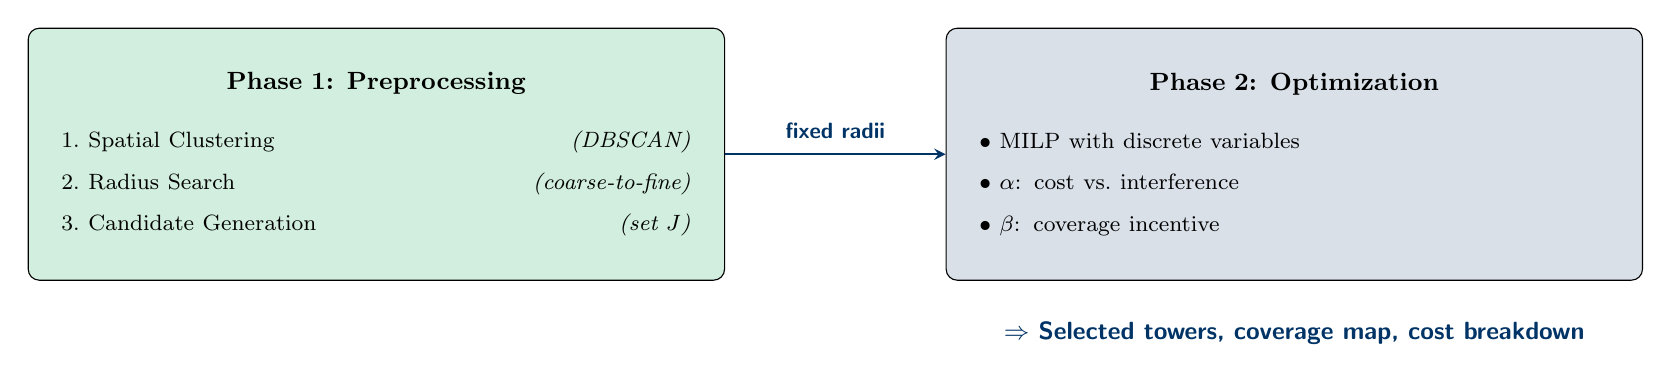
\begin{tikzpicture}[
            phasebox/.style={
                draw, rounded corners, text width=8cm, align=left,
                minimum height=3.2cm, inner sep=12pt, font=\small
            },
            arrow/.style={->, >=stealth, thick, FAUBlue},
            tag/.style={font=\footnotesize\sffamily\bfseries, FAUBlue}
        ]
            % Phase 1 Node
            \node[phasebox, fill=FAUGreen!18] (p1) {
                \centering\textbf{Phase 1: Preprocessing}\\[10pt]
                \raggedright
                {\footnotesize 1.\ Spatial Clustering \hfill \textit{(DBSCAN)}}\\[4pt]
                {\footnotesize 2.\ Radius Search \hfill \textit{(coarse-to-fine)}}\\[4pt]
                {\footnotesize 3.\ Candidate Generation \hfill \textit{(set $J$)}}
            };

            % Phase 2 Node - Increased from 1.6cm to 2.8cm to lengthen the arrow
            \node[phasebox, fill=FAUBlue!15, right=2.8cm of p1] (p2) {
                \centering\textbf{Phase 2: Optimization}\\[10pt]
                \raggedright
                {\footnotesize $\bullet$ MILP with discrete variables}\\[4pt]
                {\footnotesize $\bullet$ $\alpha$: cost vs.\ interference}\\[4pt]
                {\footnotesize $\bullet$ $\beta$: coverage incentive}
            };

            % Connection Arrow - Automatically lengthens based on the node distance
            \draw[arrow] (p1.east) -- node[above=2pt, tag] {fixed radii} (p2.west);

            % Output label - Centered relative to Phase 2 box
            \node[font=\small\sffamily\bfseries, below=0.4cm of p2, FAUBlue] (out) {
                $\Rightarrow$ Selected towers, coverage map, cost breakdown
            };
        \end{tikzpicture}
    \end{center}

    \vspace{0.15cm}
\begin{center}
    \begin{minipage}{0.95\textwidth} % adjust width here
        \begin{block}{Key Insight}
            By pre-computing the two radii in Phase~1, the MILP in Phase~2 uses only \alert{binary and continuous} variables — no non-linear terms.
        \end{block}
    \end{minipage}
    \end{center}
\end{frame}
\section[Radius Selection]{Phase 1: Radius Selection}

\begin{frame}[t]{Why DBSCAN?}{}
    \vspace{-0.3cm}
    \begin{columns}[T]
        \column{0.50\textwidth}
        \begin{block}{1. Native Noise Detection}
            \vspace{0.1cm}
            {\small K-Means and GMMs \textbf{force} every point into a cluster. DBSCAN explicitly flags isolated points as \texttt{noise} ($-1$), preventing rural outliers from distorting urban cluster geometry.}
            \vspace{0.1cm}
        \end{block}
        \vspace{0.2cm}
        \begin{block}{2. Arbitrary Density Manifolds}
            \vspace{0.1cm}
            {\small K-Means assumes \textbf{spherical} clusters with linear Voronoi boundaries. DBSCAN links points via contiguous density, capturing elongated urban corridors (e.g., Rhine-Ruhr) without imposing geometric priors.}
            \vspace{0.1cm}
        \end{block}

        \column{0.50\textwidth}
        \begin{block}{3. Physical Parameterization}
            \vspace{0.1cm}
            {\small DBSCAN replaces abstract $k$ with physically meaningful hyperparameters:}
            \begin{itemize}
                \setlength\itemsep{4pt}
                \item {\small $\varepsilon = 40\,\text{km}$ \;---\; max.\ tower signal range}
                \item {\small $\text{min\_samples} = 2$ \;---\; urban density threshold}
            \end{itemize}
            \vspace{0.1cm}
            {\small Distance metric: \textbf{haversine} (great-circle), which accounts for Earth's curvature when converting lat/lon to true ground distances.}
            \vspace{0.1cm}
        \end{block}
    \end{columns}
\end{frame}

\begin{frame}[t]{Spatial Clustering (DBSCAN)}{}
    \begin{columns}[T]
        % 1. Left Column: The cluster map
        \column{0.60\textwidth}
        \begin{center}
            \vspace{-1.3cm} 
            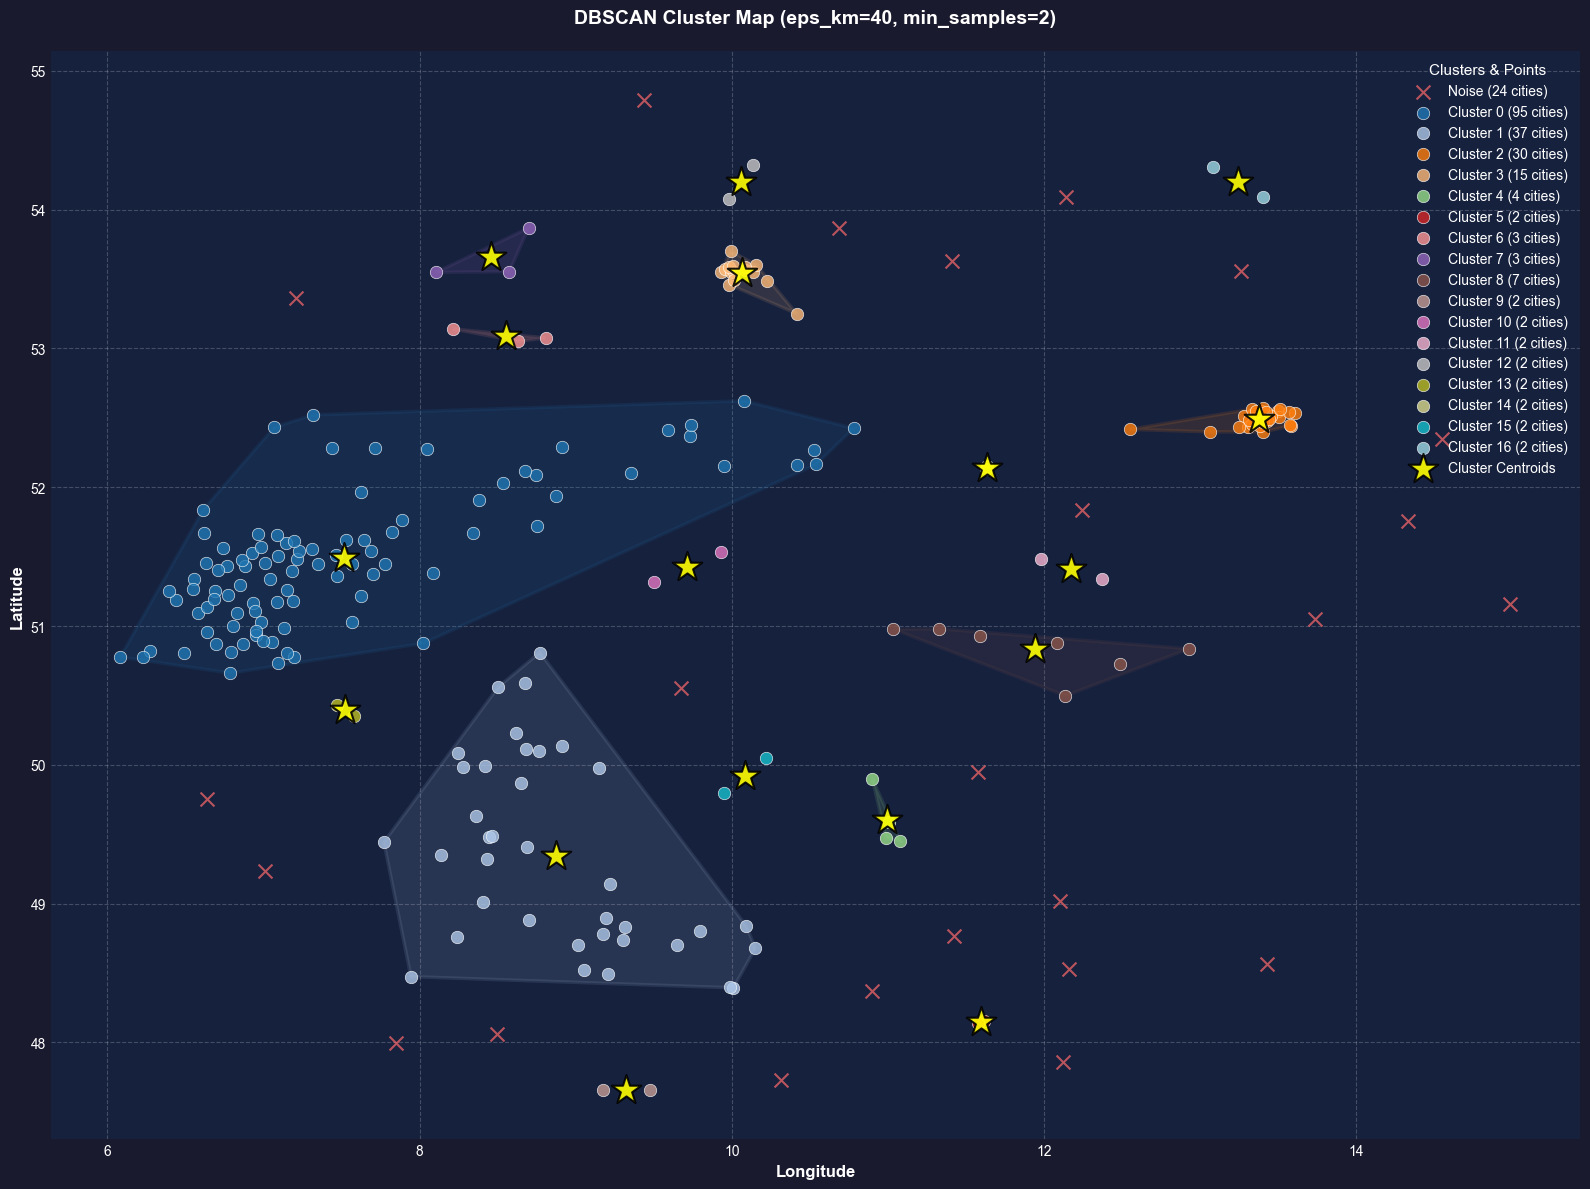
\includegraphics[width=\textwidth,height=0.80\textheight,keepaspectratio]{./images/clusters.png}
        \end{center}

        % 2. NEW Middle Column: Acts as your X-axis slider!
        \column{-1.0\textwidth}

        % This column stays completely empty to push the box to the right.
        % Increase 0.06 to push the box further right; decrease it to pull it left.
        % 3. Right Column: Contains the hyperparameter block
        \column{0.24\textwidth}
        \vspace{1.0cm} 

        \begin{block}{\centering Parameter}
            \centering
            \vspace{0.1cm}
            {\small $\varepsilon = 40\,\text{km}$} \\[4pt]
            {\small $\text{min\_samples} = 2$}
            \vspace{0.1cm}
        \end{block}
    \end{columns}
\end{frame}


\begin{frame}[t]{Computing Radius Search Bounds}{}
    \begin{center}
    \begin{minipage}{0.92\textwidth}
        \textbf{Why bounds?}\\[4pt]
        Searching all of $[5,100]$\,km is mathematically wasteful and computationally inefficient. The geographic data inherently dictates our optimal search horizon.
    \end{minipage}
    \end{center}
    \vspace{0.4cm}
    \begin{columns}[T]
        % Left Box: Lower Bound Mathematics
        \column{0.48\textwidth}
        
        \vspace{-0.45cm} % adjust to align with right block
        
        \begin{center}
        \begin{minipage}{0.92\textwidth}
            \begin{block}{Lower Bound ($r_{\min}$)}
                \begin{equation*}
                    r_{\min} = \max\!\Big(5,\; \big\lfloor \tfrac{P_{10}(\text{NN})}{2} \big\rfloor\Big)
                \end{equation*}
                \vspace{0.1cm}
                {\small Sets threshold using half the 10\textsuperscript{th} percentile of nearest-neighbor distances. Prevents over-allocating tiny towers in high-density zones.}
            \end{block}
        \end{minipage}
        \end{center}

        % Right Box: Upper Bound Mathematics
        \column{0.48\textwidth}
        \vspace{-0.45cm} % move up/down
        \begin{center}
        \begin{minipage}{0.92\textwidth} % adjust width here
            \begin{block}{Upper Bound ($r_{\max}$)}
                \begin{equation*}
                    r_{\max} = \min\!\Big(100,\; \big\lceil P_{95}(\text{pairwise}) \big\rceil\Big)
                \end{equation*}
                \vspace{0.1cm}
                {\small Sets threshold using the 95\textsuperscript{th} percentile of all global pairwise distances. Caps wasteful spatial allocation.}
            \end{block}
        \end{minipage}
        \end{center}
    \end{columns}

\end{frame}
\begin{frame}[t]{Radius Search Bounds Plot}{}
    \begin{columns}[T]
        % Dominates the left with the layout plot
        \column{0.96\textwidth}
        \begin{center}
            \vspace{-1.3cm}             
\includegraphics[width=\textwidth,height=0.80\textheight,keepaspectratio]{./images/radius_bounds_visual.png}
        \end{center}
        % Spacer column to slide box cleanly along the X-axis
        \column{0.04\textwidth}
    \end{columns}
\end{frame} 

% ==========================================
% SLIDE 4: RADIUS OPTIMIZATION METHODOLOGY
% ==========================================
\begin{frame}[t]{Coarse to Fine Radius Search}{}
    \vspace{0.2cm}
    \begin{columns}[T]
        
        % Left Column: The Mathematical Objective
        \column{0.35\textwidth}
        \begin{block}{1. Scoring Function} 
            \vspace{0.2cm}
            \begin{equation*}
                 J(r) = \frac{\overbrace{\text{cost}(r)}^{\text{installation cost}}}{\underbrace{\max\big(1,\; \overline{\text{cov}}(r)\big)}_{\text{avg.\ cities covered}}}  
            \end{equation*}
            \vspace{0.3cm}                                                    
        \end{block}

        % Right Column: The Search Strategy
        \column{0.48\textwidth}
        \begin{block}{2. Coarse-to-Fine}
            \begin{center}
                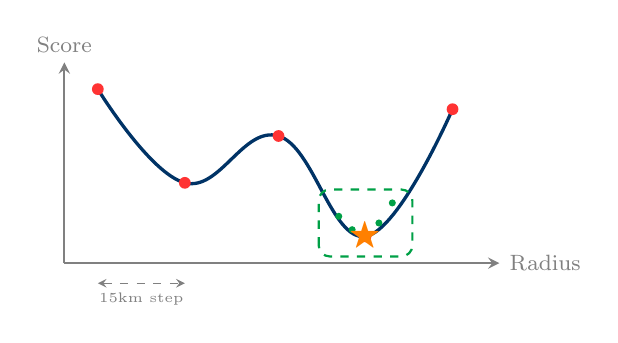
\begin{tikzpicture}[scale=0.85, >=stealth]
                    % Draw axes
                    \draw[->, gray, thick] (0,0) -- (6.5,0) node[right, font=\footnotesize] {Radius};
                    \draw[->, gray, thick] (0,0) -- (0,3.0) node[above, font=\footnotesize] {Score};

                    % Draw "Cost Landscape" curve
                    \draw[FAUBlue, very thick] plot[smooth, tension=0.7] coordinates {
                        (0.5, 2.6) (1.8, 1.2) (3.2, 1.9) (4.5, 0.4) (5.8, 2.3)
                    };

                    % Coarse Search (Big jumps)
                    \draw[<->, gray, dashed] (0.5, -0.3) -- (1.8, -0.3) node[midway, below, font=\tiny] {15km step};
                    \fill[red!80] (0.5, 2.6) circle (2.5pt);
                    \fill[red!80] (1.8, 1.2) circle (2.5pt);
                    \fill[red!80] (3.2, 1.9) circle (2.5pt);
                    \fill[red!80] (4.5, 0.4) circle (2.5pt);
                    \fill[red!80] (5.8, 2.3) circle (2.5pt);

                    % Fine Search (Zoom box)
                    \draw[FAUGreen, thick, rounded corners, dashed] (3.8, 0.1) rectangle (5.2, 1.1);
                    
                    % Little fine points around the global minimum
                    \fill[FAUGreen] (4.1, 0.7) circle (1.5pt);
                    \fill[FAUGreen] (4.3, 0.5) circle (1.5pt);
                    \fill[FAUGreen] (4.5, 0.4) circle (1.5pt);
                    \fill[FAUGreen] (4.7, 0.6) circle (1.5pt);
                    \fill[FAUGreen] (4.9, 0.9) circle (1.5pt);
                    
                    % Global Min star
                    \node[text=orange, font=\large] at (4.5, 0.4) {$\bigstar$};
                \end{tikzpicture}
            \end{center}
            
            \vspace{0.1cm}
            {\footnotesize
            \textbf{Step 1 (Coarse):} Test large 15\,km intervals (red dots) to rapidly locate the general performance "valley."\\[4pt]
            \textbf{Step 2 (Fine):} Zoom in on the top coarse result and test integer 1\,km steps within a $\pm 14$\,km window (green dots) to lock in the true global minimum ($\bigstar$).
            }
        \end{block}

    \end{columns}
\end{frame}

% ==========================================
% SLIDE 5: RADIUS OPTIMIZATION SCORES
% ==========================================
\begin{frame}[t]{Radius Optimization Scores}{}
    \begin{center}
        \vspace{0.2cm}
        
\includegraphics[width=0.95\textwidth,height=0.7\textheight,keepaspectratio]{./images/coarse_fine_score.png}
    \end{center}
\end{frame}

\section[Candidates \& Interference]{Phase 2: Candidates \& Interference}

\begin{frame}[t]{Candidate Generation}{}
    \textbf{Every city and cluster centroid becomes a possible tower location.}

    \vspace{0.2cm}
    \begin{columns}[T]
        \column{0.5\textwidth}
        \begin{block}{Candidate Sources}
            \begin{enumerate}
                \item Cluster centroids
                \item Every clustered city
                \item Every noise (isolated) city
            \end{enumerate}
        \end{block}

        \column{0.5\textwidth}
        \begin{block}{Tower Types Generated}
            At each location, we add a tower option using:
            \begin{itemize}
                \item \alert{Dense radius} ($r_{\text{dense}}$)
                \item \alert{Sparse radius} ($r_{\text{sparse}}$)
            \end{itemize}
            {\footnotesize (If the radii are equal, only one type is needed.)}
        \end{block}
    \end{columns}

    \vspace{0.2cm}
    \begin{center}
        \small
        $|J| = (\text{\# centroids} + \text{\# clustered cities} + \text{\# noise}) \;\times\; (1\text{--}2 \text{ tower types})$
    \end{center}

    \vspace{0.1cm}
    \begin{alertblock}{Why so many candidates?}
        The MILP solver decides \emph{which} candidates to activate. Over-generating candidates gives the solver flexibility; the optimization itself enforces sparsity through the cost objective.
    \end{alertblock}
\end{frame}

\begin{frame}[t]{Interference Modeling}{}
    \begin{columns}[T]
        \column{0.45\textwidth}
        \begin{block}{When Do Towers Interfere?}
            Two towers interfere if their coverage circles overlap:
            \begin{center}
                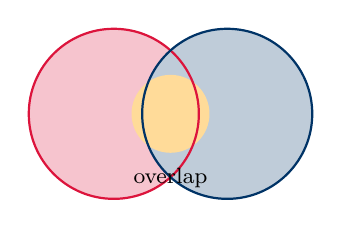
\begin{tikzpicture}[scale=0.9]
                    \fill[FAURed!25] (0,0) circle (1.2);
                    \fill[FAUBlue!25] (1.6,0) circle (1.2);
                    \fill[FAUOrange!40] (0.8,0) circle (0.55);
                    \draw[FAURed, thick] (0,0) circle (1.2);
                    \draw[FAUBlue, thick] (1.6,0) circle (1.2);
                    \node at (0.8,-0.9) {\footnotesize overlap};
                \end{tikzpicture}
            \end{center}
        \end{block}

        \column{0.55\textwidth}
        \begin{block}{Normalized Overlap Penalty}
            \begin{equation*}
                P_{pq} = \begin{cases}
                    \dfrac{R_{\text{sum}} - d}{R_{\text{sum}}}
                        & \text{if } d < R_{\text{sum}} \\[10pt]
                    0   & \text{otherwise}
                \end{cases}
            \end{equation*}
            \vspace{-0.2cm}
            {\small
            $R_{\text{sum}} = r_p + r_q$\\
            $d$ = haversine distance between towers
            }
        \end{block}
    \end{columns}

    \vspace{0.2cm}
    \begin{center}
        \small
        Pairs are pre-filtered using a \textbf{KD-tree} with query radius $2 \times r_{\max}$ \\
        $\rightarrow$ only pairs that can physically overlap are passed to the solver
    \end{center}
\end{frame}

\section{MILP Formulation}

\begin{frame}[t]{Decision Variables \& Objective}{}
    \begin{columns}[T]
        \column{0.4\textwidth}
        \begin{block}{Variables}
            \begin{tabular}{@{}c l@{}}
                \toprule
                \textbf{Var} & \textbf{Meaning} \\
                \midrule
                $x_j$   & Tower $j$ selected? \\[2pt]
                        & $\{0,1\}$ \\[6pt]
                $y_{pq}$ & Interference active? \\[2pt]
                         & $[0,1]$ \\[6pt]
                $z_i$    & City $i$ covered? \\[2pt]
                         & $\{0,1\}$ \\[6pt]
                $P_{pq}$ & norm.\ overlap penalty \\
                \bottomrule
            \end{tabular}
        \end{block}

        \column{0.6\textwidth}
        \begin{block}{Objective Function}
            \begin{equation*}
                \min \;
                \alpha\!\sum_{j} c_j x_j
                \;+\;
                (1-\alpha)\!\sum_{(p,q)} P_{pq} y_{pq}
                \;-\;
                \beta\!\sum_{i} z_i
            \end{equation*}

            \vspace{0.15cm}
            \begin{tabular}{@{}l l@{}}
                \textcolor{FAUGreen}{$\alpha$} & cost vs.\ interference trade-off \\
                \textcolor{FAUBlue}{$\beta$}  & coverage incentive \\
            \end{tabular}
        \end{block}
    \end{columns}

    \vspace{0.3cm}
    \begin{columns}[T]
        \column{0.5\textwidth}
        \begin{block}{Coverage Link}
            $z_i \;\le\; \displaystyle\sum_{j \text{ covering } i} x_j$
            \vspace{4pt}

            {\footnotesize A city counts as covered only if at least one tower that covers it is selected.}
        \end{block}

        \column{0.5\textwidth}
        \begin{block}{Interference Linearization}
            $y_{pq} \;\le\; x_p,\; y_{pq} \;\le\; x_q$\\
            $y_{pq} \;\ge\; x_p + x_q - 1$
            \vspace{4pt}

            {\footnotesize Three linear constraints encode $y_{pq} = x_p \land x_q$.}
        \end{block}
    \end{columns}
\end{frame}

\begin{frame}[t]{Why $\alpha$ and $\beta$ Matter}{}
    \begin{columns}[T]
        \column{0.5\textwidth}
        \begin{block}{$\alpha$: Cost vs.\ Interference}
            \begin{itemize}
                \item $\alpha = 1.0$: minimize cost, ignore interference
                \item $\alpha = 0.0$: minimize interference, ignore cost
                \item $\alpha = 0.5$: balance both equally
            \end{itemize}
            {\footnotesize Default in our runs: $\alpha = 0.5$}
        \end{block}

        \column{0.5\textwidth}
        \begin{block}{$\beta$: Coverage Incentive}
            \begin{itemize}
                \item Without $\beta$: cheapest solution is 0 towers
                \item $\beta > 0$: rewards covering more cities
                \item Higher $\beta$ pushes coverage toward 100\%
            \end{itemize}
            {\footnotesize Default in our runs: $\beta = 0.8$}
        \end{block}
    \end{columns}

    \vspace{0.3cm}
    \begin{alertblock}{Practical Effect}
        With $\alpha=0.5$, $\beta=0.8$: the solver finds a solution with \alert{99.6\% coverage} while keeping \alert{interference at 1.58\%} of total coverage area — a strong balance between the three competing objectives.
    \end{alertblock}
\end{frame}

\section{Results}

% ==========================================
% SLIDE 1: COMPUTATIONAL RESULTS (DATA)
% ==========================================
\begin{frame}[t]{Computational Results: Key Metrics}{}

    \begin{block}{\centering Run Configuration}
        \centering
        \vspace{0.1cm}
        {\small $\varepsilon = 40$\,km \hspace{0.5cm} min\_samples $=2$ \hspace{0.5cm} $\alpha = 0.5$ \hspace{0.5cm} $\beta = 0.22$}
        \vspace{0.1cm}
    \end{block}

    \vspace{0.3cm}
    \begin{columns}[T]
        \column{0.48\textwidth}
        \begin{block}{Phase 1: Search Space \& Clustering}
            \centering
            \renewcommand{\arraystretch}{1.3}
            \begin{tabular}{@{}l r@{}}
                \toprule
                \textbf{Metric}             & \textbf{Value} \\
                \midrule
                Dense radius                & 27\,km \\
                Sparse radius               & 89\,km \\
                Clusters found              & 17 \\
                Noise cities (isolated)     & 24 \\
                Candidates generated        & 506 \\
                \bottomrule
            \end{tabular}
        \end{block}

        \column{0.48\textwidth}
        \begin{block}{Phase 2: Optimization Outcome}
            \centering
            \renewcommand{\arraystretch}{1.3}
            \begin{tabular}{@{}l r@{}}
                \toprule
                \textbf{Metric}             & \textbf{Value} \\
                \midrule
                Towers selected             & \textbf{52} \\
                Coverage ratio              & \textbf{100\%} \\
                Total tower cost            & 91.18 \\
                Overlap penalty             & 1.96\% \\
                Solver status               & Optimal \\
                \bottomrule
            \end{tabular}
        \end{block}
    \end{columns}
\end{frame}

% ==========================================
% SLIDE 2: FINAL NETWORK TOPOLOGY (VISUAL)
% ==========================================
\begin{frame}[t]{Optimized 6G Network Topology}{}
    \begin{columns}[T]
        \column{0.70\textwidth}
        \begin{center}
            \vspace{-0.4cm}
            
\includegraphics[width=\textwidth,height=0.78\textheight,keepaspectratio]{./images/results vis.png}
        \end{center}

        \column{0.08\textwidth}

        \column{0.22\textwidth}
        \begin{block}{\centering Final KPIs}
            \centering
            \vspace{0.1cm}
            {\small \textbf{Towers Built:}\\ \alert{52}} \\[8pt]
            {\small \textbf{Coverage:}\\ \alert{100\%}} \\[8pt]
            {\small \textbf{Overlap:}\\ \alert{$<$ 2\%}}
            \vspace{0.1cm}
        \end{block}
    \end{columns}
\end{frame}

\section[Limitations \& Outlook]{Limitations \& Future Work}

\begin{frame}[t]{Limitations \& Future Work}{}
    \begin{columns}[T]
        \column{0.48\textwidth}
        \begin{alertblock}{Current Limitations}
            \begin{itemize}
                \item \textbf{Two radii only.} Some towers would benefit from intermediate sizes. Pre-selecting exactly two values reduces flexibility.

                \vspace{0.2cm}
                \item \textbf{DBSCAN sensitivity.} Cluster count and noise assignment depend heavily on $\varepsilon$ and min\_samples. A poor clustering can degrade radius quality.
            \end{itemize}
        \end{alertblock}

        \column{0.48\textwidth}
        \begin{block}{Planned Improvements}
            \begin{itemize}
                \item \textbf{Local radius refinement.} After MILP selects tower locations, run gradient-based NLP to fine-tune each tower's radius independently.

                \vspace{0.2cm}
                \item \textbf{Automated clustering.} Grid-search over DBSCAN parameters to find the configuration that yields the best MILP objective.

                \vspace{0.2cm}
                \item \textbf{Additional tower types.} Extend from 2 to $k$ radii types with a minimal increase in candidate set size.
            \end{itemize}
        \end{block}
    \end{columns}
\end{frame}


\end{document}
